%%%%%%%%%%%%%%%%%%%%%%%%%%%%%%%%%%%%%%%%%%%%%%%%%%%
%% P3: Phenomenology of Particle Physics                         
%%
%% Author:  André Rubbia                   		 
%%
%% Figure 2.17 Wavelength spectra of X-rays scattered at $45^\circ$, $90^\circ$, and $135^\circ$  by a carbon (graphite) foil, compared to the original $K\alpha$-line.
%%
%% This work is licensed under the Creative Commons Attribution 4.0 International License. 
%% To view a copy of this license, visit http://creativecommons.org/licenses/by/4.0/ or 
%% send a letter to Creative Commons, PO Box 1866, Mountain View, CA 94042, USA.
%%
%% Data taken with permission from A. H. Compton, ``The spectrum of scattered $X$-rays,''  Phys. Rev. , vol. 22,
%%  pp. 409--413, Nov 1923. 
%%
%%%%%%%%%%%%%%%%%%%%%%%%%%%%%%%%%%%%%%%%%%%%%%%%%%%

\documentclass[a4paper,10pt]{article}

\usepackage[T1]{fontenc}
\usepackage[utf8]{inputenc}
\usepackage{lmodern}
\usepackage[labelfont=bf]{caption}
\usepackage{upgreek}
\usepackage{amssymb}
\usepackage{amsmath}

\usepackage{tikz}
\usepackage{pgfplots}
\pgfplotsset{compat=1.17}
\usepgfplotslibrary{ternary}
\usepgfplotslibrary{fillbetween}
\usepgfplotslibrary{external}


\def\d{\mathrm{d}}

\begin{document}

%%%%%%%%%%%%%%%   FIGURE  %%%%%%%%%%%%%%%%%%%%%%%%%%%%%%
\begin{figure}[htb]
\begin{center}
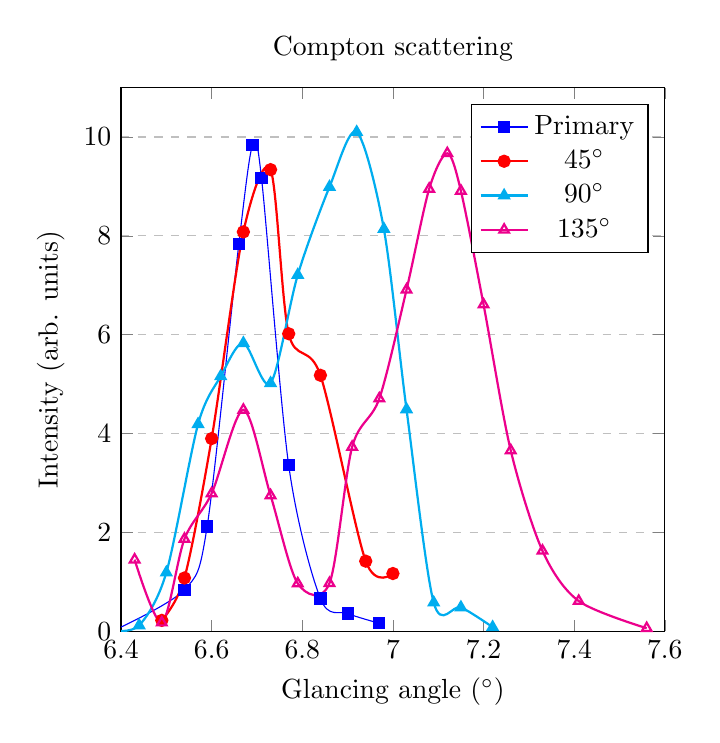
\begin{tikzpicture}[scale=1]
\begin{axis}[
    width=0.7\textwidth,
    height=0.7\textwidth,
    title={Compton scattering},
    xlabel={Glancing angle ($^\circ$)},
    ylabel={Intensity (arb. units)},
    xmin=6.4, xmax=7.6,
    ymin=0, ymax=11,
    legend pos=north east,
    ymajorgrids=true,
    grid style=dashed,
]
\addplot[
    color=blue,smooth,
    mark=square*,
    ]
    coordinates {
%%primary Kalpha line Molybdenum
(6.38,0.)
(6.54,0.843)
(6.59,2.12)
(6.66,7.84)
(6.69,9.83)
(6.71,9.17)
(6.77,3.36)
(6.84,0.663)
(6.90,0.362)
(6.97,0.164)
    };
\addplot[
    color=red, smooth,thick,
    mark=*,
    ]
    coordinates {
% scattered by graphite at 45deg
(6.49,0.222)
(6.54,1.08)
(6.60,3.90)
(6.67,8.08)
(6.73,9.34)
(6.77,6.02)
(6.84,5.18)
(6.94,1.42)
(7.00,1.17)
    };

\addplot[
    color=cyan, smooth,thick,
    mark=triangle*,
    ]
    coordinates {
 % scattered by graphite at 90deg
(6.38,0.0143)
(6.44,0.121)
(6.50,1.19)
(6.57,4.19)
(6.62,5.16)
(6.67,5.83)
(6.73,5.02)
(6.79,7.21)
(6.86,8.99)
(6.92,10.1)
(6.98,8.14)
(7.03,4.49)
(7.09,0.582)
(7.15,0.485)
(7.22,0.0852)
    };
\addplot[
    color=magenta, smooth,thick,
    mark=triangle,
    ]
    coordinates {
% scattered by graphite at 135deg
(6.43,1.45)
(6.49,0.177)
(6.54,1.87)
(6.60,2.79)
(6.67,4.48)
(6.73,2.75)
(6.79,0.968)
(6.86,0.974)
(6.91,3.73)
(6.97,4.71)
(7.03,6.91)
(7.08,8.95)
(7.12,9.67)
(7.15,8.91)
(7.20,6.61)
(7.26,3.66)
(7.33,1.63)
(7.41,0.613)
(7.56,0.0637)
    };

         \legend{Primary, $45^\circ$,$90^\circ$,$135^\circ$}

\end{axis}
\end{tikzpicture}
\caption{Wavelength spectra of $X$-rays scattered at $45^\circ$,
$90^\circ$, and $135^\circ$  by a carbon (graphite) foil, compared to the original
$K\alpha$-line.}
\end{center}
\end{figure}
%%%%%%%%%%%%%%%   END FIGURE  %%%%%%%%%%%%%%%%%%%%%%%%%%%%%%
\end{document}
